%\thispagestyle{myheadings}
\section{Invited Talk: Dan Jurafsky}
\index{Jurafsky, Dan}

\begin{center}
\begin{Large}
{\bfseries\Large ``Does This Vehicle Belong to You''? Processing the Language of Policing for Improving Police-Community Relations}\vspace{1em}\par
\end{Large}

%% \begin{center}
%%   \begin{tabular}{m{1in}b{1in}}
%%     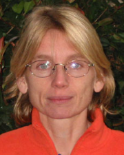
\includegraphics[width=1in]{content/monday/cortes-headshot.png}
%%     & {\bfseries Corinna Cortes} \newline Google Research, NY
%%   \end{tabular}
%% \end{center}

\daydateyear, 9:00--10:10am \vspace{1em}\\
\PlenaryLoc \\
\vspace{1em}\par
%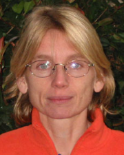
\includegraphics[height=100px]{content/monday/cortes-headshot.png}
\end{center}

\noindent
{\bfseries Abstract:} Police body-cameras have the potential to play an important
role in understanding and improving police-community relations.
In this talk I describe a series of studies conducted by our
large interdisciplinary team at Stanford that use speech and
natural language processing on body-camera recordings to model the interactions
between police officers and community members in traffic stops.
We use text and speech features to automatically measure linguistic aspects of the interaction,
from discourse factors like conversational structure to social factors like respect.
I describe the differences we find in the language directed toward black versus white community members,
and offer suggestions for how these findings can be used to help improve the fraught relations between
police officers and the communities they serve.

\vspace{3em}\par 

\vfill
\noindent

{\bfseries Biography:} Dan Jurafsky is Professor and Chair of Linguistics and Professor
  of Computer Science, at Stanford University.  His research has
  focused on the extraction of meaning, intention, and affect from
  text and speech, on the processing of Chinese, and on applying
  natural language processing to the cognitive and social sciences.
  Dan's deep interest in NLP education led him to co-write with Jim
  Martin the widely-used textbook "Speech and Language Processing”
  (whose 3rd edition is in (slow) progress) and co-teach with Chris Manning
  the first massive open online class on natural language processing.
  Dan was the recipient of the 2002 MacArthur Fellowship and is a
  2015 James Beard Award Nominee for his book, "The Language of Food:
  A Linguist Reads the Menu".

\newpage
